% Options for packages loaded elsewhere
\PassOptionsToPackage{unicode}{hyperref}
\PassOptionsToPackage{hyphens}{url}
%
\documentclass[
]{article}
\usepackage{amsmath,amssymb}
\usepackage{iftex}
\ifPDFTeX
  \usepackage[T1]{fontenc}
  \usepackage[utf8]{inputenc}
  \usepackage{textcomp} % provide euro and other symbols
\else % if luatex or xetex
  \usepackage{unicode-math} % this also loads fontspec
  \defaultfontfeatures{Scale=MatchLowercase}
  \defaultfontfeatures[\rmfamily]{Ligatures=TeX,Scale=1}
\fi
\usepackage{lmodern}
\ifPDFTeX\else
  % xetex/luatex font selection
\fi
% Use upquote if available, for straight quotes in verbatim environments
\IfFileExists{upquote.sty}{\usepackage{upquote}}{}
\IfFileExists{microtype.sty}{% use microtype if available
  \usepackage[]{microtype}
  \UseMicrotypeSet[protrusion]{basicmath} % disable protrusion for tt fonts
}{}
\makeatletter
\@ifundefined{KOMAClassName}{% if non-KOMA class
  \IfFileExists{parskip.sty}{%
    \usepackage{parskip}
  }{% else
    \setlength{\parindent}{0pt}
    \setlength{\parskip}{6pt plus 2pt minus 1pt}}
}{% if KOMA class
  \KOMAoptions{parskip=half}}
\makeatother
\usepackage{xcolor}
\usepackage[margin=1in]{geometry}
\usepackage{graphicx}
\makeatletter
\def\maxwidth{\ifdim\Gin@nat@width>\linewidth\linewidth\else\Gin@nat@width\fi}
\def\maxheight{\ifdim\Gin@nat@height>\textheight\textheight\else\Gin@nat@height\fi}
\makeatother
% Scale images if necessary, so that they will not overflow the page
% margins by default, and it is still possible to overwrite the defaults
% using explicit options in \includegraphics[width, height, ...]{}
\setkeys{Gin}{width=\maxwidth,height=\maxheight,keepaspectratio}
% Set default figure placement to htbp
\makeatletter
\def\fps@figure{htbp}
\makeatother
\setlength{\emergencystretch}{3em} % prevent overfull lines
\providecommand{\tightlist}{%
  \setlength{\itemsep}{0pt}\setlength{\parskip}{0pt}}
\setcounter{secnumdepth}{-\maxdimen} % remove section numbering
% definitions for citeproc citations
\NewDocumentCommand\citeproctext{}{}
\NewDocumentCommand\citeproc{mm}{%
  \begingroup\def\citeproctext{#2}\cite{#1}\endgroup}
\makeatletter
 % allow citations to break across lines
 \let\@cite@ofmt\@firstofone
 % avoid brackets around text for \cite:
 \def\@biblabel#1{}
 \def\@cite#1#2{{#1\if@tempswa , #2\fi}}
\makeatother
\newlength{\cslhangindent}
\setlength{\cslhangindent}{1.5em}
\newlength{\csllabelwidth}
\setlength{\csllabelwidth}{3em}
\newenvironment{CSLReferences}[2] % #1 hanging-indent, #2 entry-spacing
 {\begin{list}{}{%
  \setlength{\itemindent}{0pt}
  \setlength{\leftmargin}{0pt}
  \setlength{\parsep}{0pt}
  % turn on hanging indent if param 1 is 1
  \ifodd #1
   \setlength{\leftmargin}{\cslhangindent}
   \setlength{\itemindent}{-1\cslhangindent}
  \fi
  % set entry spacing
  \setlength{\itemsep}{#2\baselineskip}}}
 {\end{list}}
\usepackage{calc}
\newcommand{\CSLBlock}[1]{\hfill\break\parbox[t]{\linewidth}{\strut\ignorespaces#1\strut}}
\newcommand{\CSLLeftMargin}[1]{\parbox[t]{\csllabelwidth}{\strut#1\strut}}
\newcommand{\CSLRightInline}[1]{\parbox[t]{\linewidth - \csllabelwidth}{\strut#1\strut}}
\newcommand{\CSLIndent}[1]{\hspace{\cslhangindent}#1}
\ifLuaTeX
  \usepackage{selnolig}  % disable illegal ligatures
\fi
\usepackage{bookmark}
\IfFileExists{xurl.sty}{\usepackage{xurl}}{} % add URL line breaks if available
\urlstyle{same}
\hypersetup{
  pdftitle={Vivid Volcano: Empowering Non-Bioinformaticians to Analyze Pre-Processed Omics Data},
  pdfauthor={Tomasz M.Stępkowski},
  hidelinks,
  pdfcreator={LaTeX via pandoc}}

\title{Vivid Volcano: Empowering Non-Bioinformaticians to Analyze
Pre-Processed Omics Data}
\author{Tomasz M.Stępkowski}
\date{}

\begin{document}
\maketitle

DatViseR - Freelance R programmer, Warsaw, Poland

2025-03-26

key words: R ,R Shiny, Bioinformatics, Omics, Proteomics,
Transcriptomics, Genomics , Volcano Plot, Gene Set Enrichment Analysis,
Omics data visualisation, Omics data exploration

\section{Summary}\label{summary}

Vivid Volcano is an R Shiny web application -- an intuitive tool that
helps experimental scientists with no bioinformatics background explore
and analyze pre-processed omics data. It enables users to perform
crucial bioinformatic analyses without the help of specialists. With
Vivid Volcano, one can create highly customizable, publication-ready
volcano plots and perform comprehensive data exploration, and gene
ontology (GO) enrichment analysis. Users can download variously
formatted publication-ready plots and neatly formatted tables that
adhere to scientific standards. Vivid Volcano empowers both exploratory
and explanatory data analysis.

\section{Statement of need}\label{statement-of-need}

Modern biological research relies heavily on omics technologies
(genomics, proteomics, transcriptomics, etc.) that generate large,
complex datasets requiring specialized analysis and processing by
bioinformaticians -- experts with a unique combination of programming,
statistics, and data science skills blended with biology domain
knowledge(Manzoni et al. 2018) . These experts build analysis pipelines
which produce pre-processed data conveying metadata on experiments and
statistical results for the changes in expression of thousands of
proteins, genes, etc. However, to draw valid biological conclusions,
this pre-processed data must be explored and explained by subdomain
experts who are usually experimentalists who designed the experiments
but often do not have strong computational skills enabling them to
effectively explore data and visualize crucial conclusions. Despite the
widespread adoption of omics technologies in biological research, many
experimental scientists struggle with data analysis due to technical
barriers and communication challenges between computational and
experimental disciplines, even with bioinformatician support.

Vivid Volcano was designed with two basic aims: 1. Empowering
experimental biologists with a tool that can help them explore and
analyze pre-processed omics data on their own 2. Lowering the workload
for bioinformaticians who can focus on more statistically and
computationally challenging tasks such as integration of complex
multiomics data

Vivid Volcano addresses a critical need in the biological research
community by empowering wet-lab scientists to independently analyze and
interpret preprocessed omics data without requiring programming
expertise or extensive bioinformatics support. The application provides
an accessible interface for uploading and diagnosing preprocessed omics
data, performing customized statistical analyses including gene set
enrichment analysis across more than 8,000 GO categories, and generating
publication-ready visualizations. Unlike many existing tools, Vivid
Volcano maintains a simple and efficient design that does not rely on
Bioconductor libraries, making it more accessible and easier to
maintain. Vivid Volcano was designed to provide a smooth and intuitive
user experience. For more advanced users who would like to validate the
under-the-hood processes, the application also implements a custom
process log system that tracks data processing outcomes, facilitating
debugging and enabling analysis of app functionality. These features
collectively enable experimental biologists to gain deeper insights from
their omics data, accelerate research workflows, and produce
publication-quality outputs without advanced computational skills.

Vivid Volcano has been designed based on firsthand experience with the
challenges faced by experimental biologists working with omics data and
aims to provide comprehensive yet accessible solutions for generating
publication-ready outputs from preprocessed omics datasets.

The application is available online at
\url{https://datviser-vivid-volcano.share.connect.posit.cloud/}, making
it readily accessible to researchers worldwide.

\section{Technical description and
implementation}\label{technical-description-and-implementation}

Vivid Volcano is built as a modular R Shiny web application leveraging
the robust reactive programming model that Shiny provides. The
application architecture is characterized by clear separation between
the user interface, server logic, and data processing components. The
core functionality is implemented in R, with CSS for custom styling and
JavaScript for enhanced interactivity. The application utilizes several
key R packages, among others: shiny for the web framework (Chang et al.
2024) , shiny.semantic(Stachura et al. 2024) for user interface
(citation), DT for interactive data tables(Xie, Cheng, and Tan 2024) ,
ggplot2(Wickham 2016) and plotly(Sievert 2020) for generating
publication-quality visualizations(citations), GT for publication ready
tables(Iannone et al. 2024) and shinyjs(Attali 2021) and
shinyalert(Attali and Edwards 2024) for improved user experience . For
statistical analysis, the application employs basic R operations and
custom functions for ontology enrichment that don't rely on Bioconductor
dependencies, making the application more accessible and maintainable.
Data processing is handled through dplyr, tidyr, and other tidyverse
packages which provide efficient data manipulation
capabilities{[}Wickham et al. (2023){]}(Wickham, Vaughan, and Girlich
2024) . The application implements a custom logging system to track all
data transformations, ensuring transparency and reproducibility of
results. Vivid Volcano's modular design allows for straightforward
extension and maintenance, with clearly separated UI modules for data
upload, visualization, statistical analysis, and results export. The
application is deployed on Posit Connect Cloud (formerly RStudio Cloud),
making it accessible via web browser without requiring local
installation.

\section{Statistics and Limitations}\label{statistics-and-limitations}

Vivid Volcano takes an innovative approach to gene set enrichment
analysis by prioritizing speed and accessibility without sacrificing
essential statistical rigor. Unlike many similar tools, it does not rely
on Bioconductor libraries, which makes the application significantly
faster, more lightweight, and better suited for web-based deployment and
non-technical user. This independence from heavy computational
dependencies allows researchers to analyze data quickly in a browser
interface, without requiring specialized software installation. Standard
Bioconductor packages typically operate on complex data structures and
specialized objects that, while powerful for comprehensive analyses,
introduce significant computational overhead unsuitable for responsive
web applications. Vivid Volcano addresses this limitation by storing
crucial Gene Ontology information in highly optimized binary parquet
files---a column-oriented data format designed for efficient querying
and retrieval. This streamlined approach provides rapid access to
approximately 8,000 GO categories and their gene associations without
the memory and processing demands of traditional Bioconductor
implementations. Vivid Volcano's gene set enrichment analysis is based
on the hypergeometric test, a robust method for determining whether
specific gene sets are overrepresented among regulated genes. This test
calculates the probability of observing the particular overlap between
regulated genes and genes belonging to specific GO categories by chance.
By comparing the actual number of regulated genes in a category against
what would be expected randomly, the test provides a measure of
enrichment. The implementation utilizes four key values: the total genes
detected in the experiment, the number of genes in a given GO category,
the total regulated genes in the experiment, and the number of regulated
genes found in that category. To control false positives, Vivid Volcano
implements multiple safeguards: multiple testing correction,
customizable significance thresholds, fold enrichment filtering, and
gene set size limitations that exclude very small or overly broad
categories. The application also transparently addresses the limitations
of standard p-value adjustment methods when applied to Gene Ontology
data. As noted in the footnotes of the results tables, traditional
approaches like Benjamini--Hochberg (BH) were not developed specifically
for hierarchical data structures like the GO tree. Thus, biologically
meaningful ``parent'' categories might be missed when BH over-corrects
due to many related, statistically significant ``child'' categories.
Conversely, overly broad categories can become significant when BH
under-corrects, driven primarily by very highly significant specialized
subcategories.

Instead of implementing complex solutions that might impede performance
and confuse users, Vivid Volcano offers a smooth user experience while
clearly communicating methodological considerations. The application
provides a pragmatic balance between statistical precision and practical
utility, making sophisticated analyses accessible to researchers without
extensive bioinformatics expertise.

\section{Figures}\label{figures}

\begin{figure}
\centering
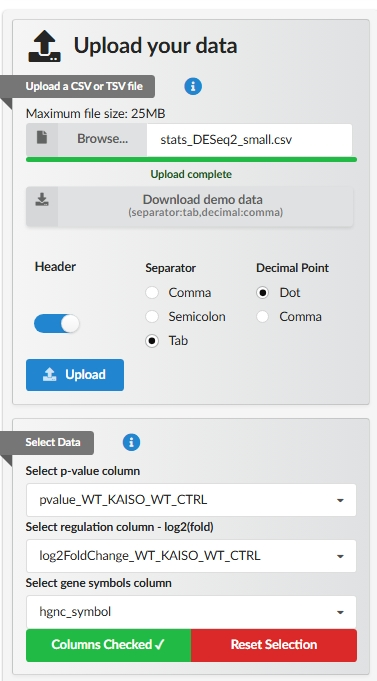
\includegraphics[width=2.51042in,height=\textheight]{Paper_figures/Data_upload_and_curation.jpeg}
\caption{Fig.1. Data upload and data select and curation modules of the
Vivid Volcano application}
\end{figure}

\begin{figure}
\centering
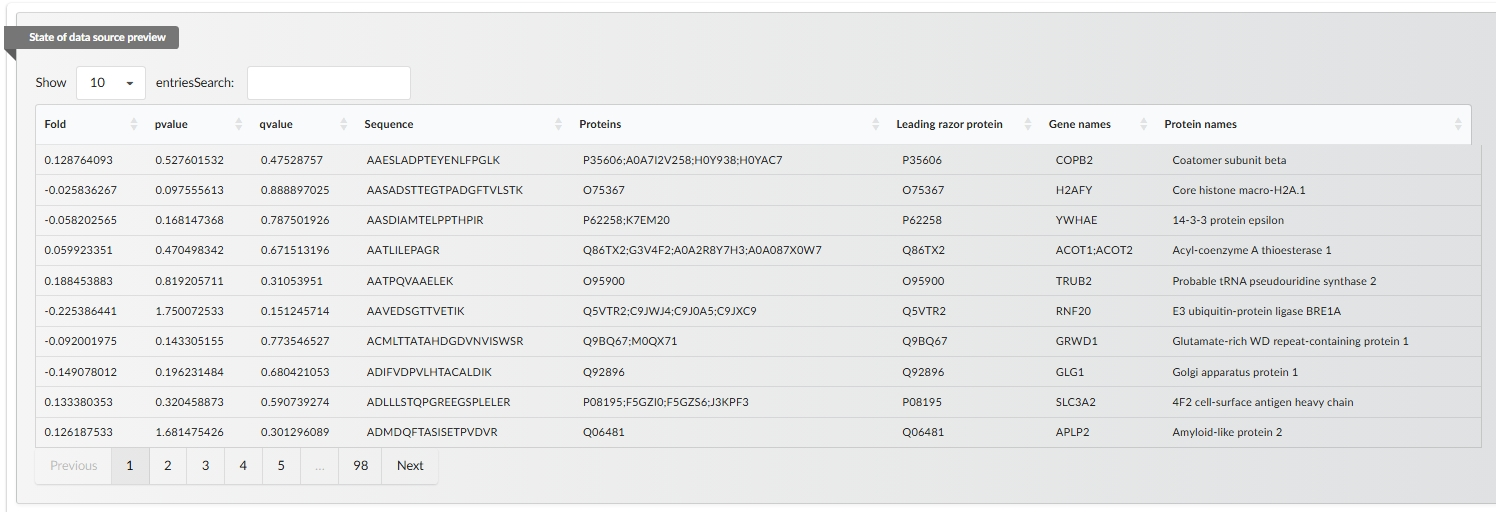
\includegraphics{Paper_figures/Data_preview.jpeg}
\caption{Fig.2. Interactive datatable preview of the analyzed data in
the Vivid Volcano application.}
\end{figure}

\begin{figure}
\centering
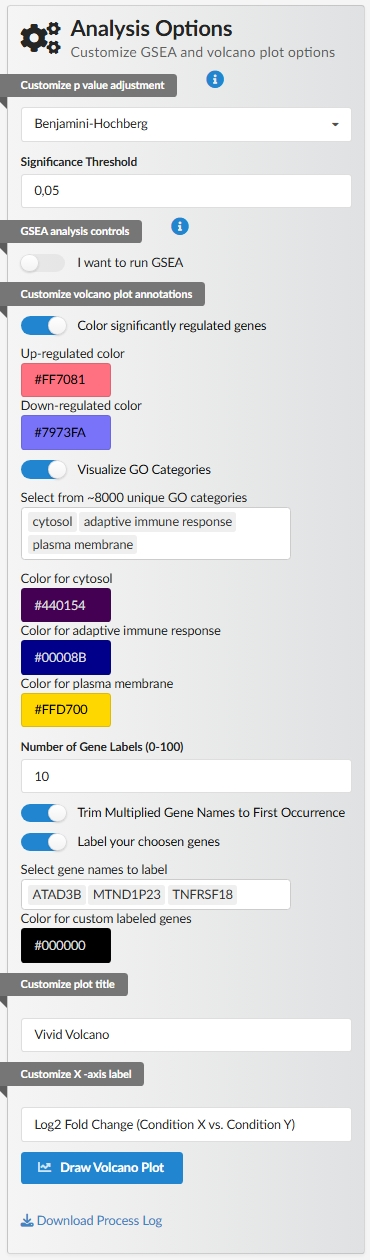
\includegraphics[width=2.4375in,height=\textheight]{Paper_figures/Volcano_plot_customisation_options.jpeg}
\caption{Fig.3.Volcano plot customisation options in the Vivid Volcano
application}
\end{figure}

\begin{figure}
\centering
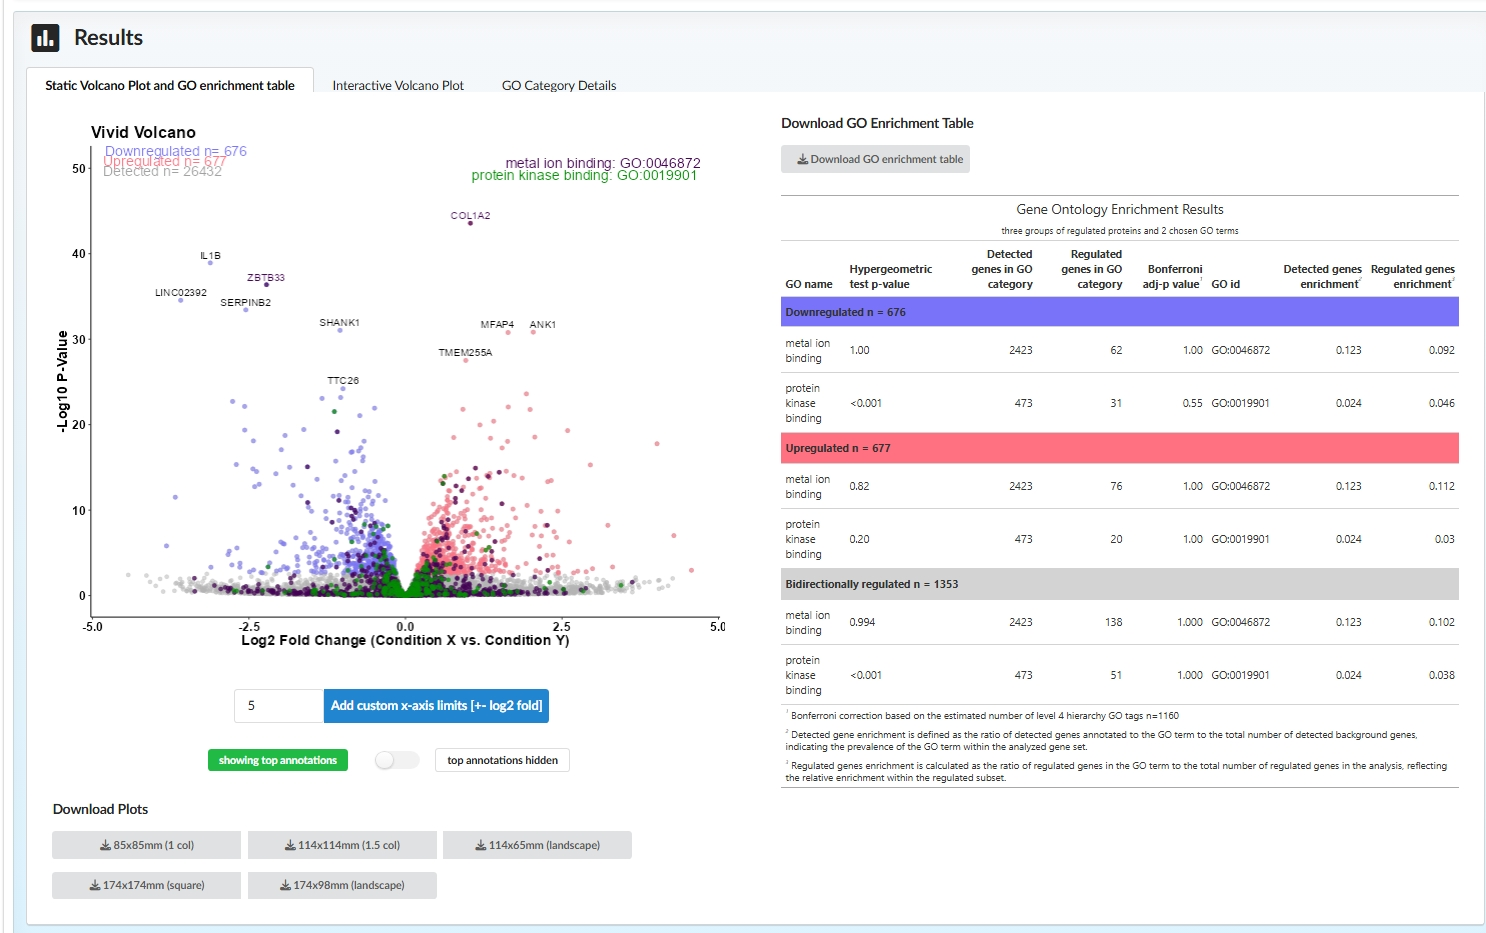
\includegraphics{Paper_figures/Volcano.jpeg}
\caption{Fig.4. Volcano plot and publication ready tabular results
generated with Vivid Volcano application}
\end{figure}

\begin{figure}
\centering
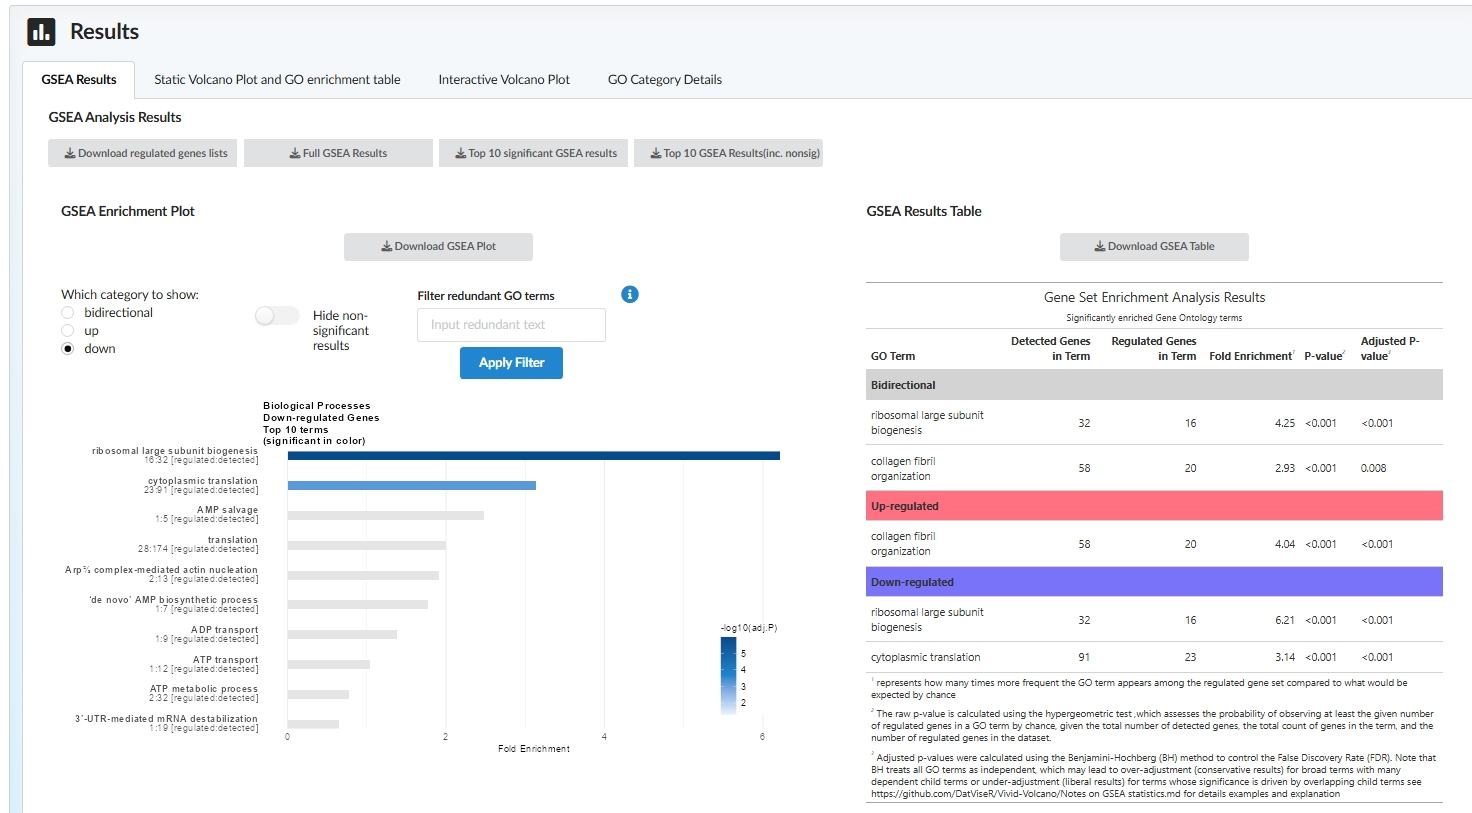
\includegraphics{Paper_figures/GSEA.jpeg}
\caption{Fig.5. The results of Gene Set Enrichment analysis performed
with VIvid Volcano application}
\end{figure}

\section{Acknowledgements}\label{acknowledgements}

The author would like to thank all the beta users especially Konrad
Kowalski and dr Anna Marusiak for their feedback and suggestions that
helped to improve the application.

The author would like to thank the developers of R, RStudio, and the R
community for providing the tools and support necessary to create this
work.

\section{AI statement}\label{ai-statement}

The author used Claude Sonnet 3.7 to copy edit and proofread the
manuscript. The author has reviewed generated fragments and corrections
to the text to ensure its accuracy and coherence.

\section*{References}\label{references}
\addcontentsline{toc}{section}{References}

\phantomsection\label{refs}
\begin{CSLReferences}{1}{0}
\bibitem[\citeproctext]{ref-shinyjs}
Attali, Dean. 2021. {``Shinyjs: Easily Improve the User Experience of
Your Shiny Apps in Seconds.''} \url{https://deanattali.com/shinyjs/}.

\bibitem[\citeproctext]{ref-shinyalert}
Attali, Dean, and Tristan Edwards. 2024. {``Shinyalert: Easily Create
Pretty Popup Messages (Modals) in 'Shiny'.''}
\url{https://github.com/daattali/shinyalert}.

\bibitem[\citeproctext]{ref-shiny}
Chang, Winston, Joe Cheng, JJ Allaire, Carson Sievert, Barret Schloerke,
Yihui Xie, Jeff Allen, Jonathan McPherson, Alan Dipert, and Barbara
Borges. 2024. {``Shiny: Web Application Framework for r.''}
\url{https://CRAN.R-project.org/package=shiny}.

\bibitem[\citeproctext]{ref-gt}
Iannone, Richard, Joe Cheng, Barret Schloerke, Ellis Hughes, Alexandra
Lauer, JooYoung Seo, Ken Brevoort, and Olivier Roy. 2024. {``Gt: Easily
Create Presentation-Ready Display Tables.''}
\url{https://gt.rstudio.com}.

\bibitem[\citeproctext]{ref-manzoni2018}
Manzoni, Claudia, Demis A Kia, Jana Vandrovcova, John Hardy, Nicholas W
Wood, Patrick A Lewis, and Raffaele Ferrari. 2018. {``Genome,
Transcriptome and Proteome: The Rise of Omics Data and Their Integration
in Biomedical Sciences.''} \emph{Briefings in Bioinformatics} 19 (2):
286--302. \url{https://doi.org/10.1093/bib/bbw114}.

\bibitem[\citeproctext]{ref-plotly}
Sievert, Carson. 2020. {``Interactive Web-Based Data Visualization with
r, Plotly, and Shiny.''} \url{https://plotly-r.com}.

\bibitem[\citeproctext]{ref-shiny.semantic}
Stachura, Filip, Dominik Krzeminski, Krystian Igras, Adam Forys, Paweł
Przytuła, Jakub Chojna, Olga Mierzwa-Sulima, Jakub Nowicki, and
Tymoteusz Makowski. 2024. {``Shiny.semantic: Semantic UI Support for
Shiny.''} \url{https://appsilon.github.io/shiny.semantic/}.

\bibitem[\citeproctext]{ref-ggplot2}
Wickham, Hadley. 2016. {``Ggplot2: Elegant Graphics for Data
Analysis.''} \url{https://ggplot2.tidyverse.org}.

\bibitem[\citeproctext]{ref-dplyr}
Wickham, Hadley, Romain François, Lionel Henry, Kirill Müller, and Davis
Vaughan. 2023. {``Dplyr: A Grammar of Data Manipulation.''}
\url{https://dplyr.tidyverse.org}.

\bibitem[\citeproctext]{ref-tidyr}
Wickham, Hadley, Davis Vaughan, and Maximilian Girlich. 2024. {``Tidyr:
Tidy Messy Data.''} \url{https://tidyr.tidyverse.org}.

\bibitem[\citeproctext]{ref-DT}
Xie, Yihui, Joe Cheng, and Xianying Tan. 2024. {``DT: A Wrapper of the
JavaScript Library 'DataTables'.''} \url{https://github.com/rstudio/DT}.

\end{CSLReferences}

\end{document}
